\documentclass[pdflatex,compress,mathserif]{beamer}

%\usetheme[dark,framenumber,totalframenumber]{ElektroITK}
\usetheme[darktitle,framenumber,totalframenumber]{ElektroITK}

\usepackage[utf8]{inputenc}
\usepackage[T1]{fontenc}
\usepackage{lmodern}
\usepackage[bahasai]{babel}
\usepackage{amsmath}
\usepackage{amsfonts}
\usepackage{amssymb}
\usepackage{graphicx}
\usepackage{multicol}

\title{Digital Signal Processing}
\subtitle{The discrete-time Fourier transform}

\author{Mifta Nur Farid}

\begin{document}

\maketitle

\begin{frame}
	\frametitle{Frequency Response of LSI}
	\begin{itemize}
		\item Complex exponential input ($ e^{j \omega n} $) $\rightarrow$ complex exponential sequence output with same complex frequency ($ e^{j \omega n} $), but with a change in amplitude.
		\item The change in amplitude is the function ($ H(e^{j\omega}) $) = frequency response of the system
		\[ e^{j \omega n} \rightarrow H(e^{j\omega}) e^{j \omega n} \]
		\item Frequency response ($ H(e^{j\omega}) $) in terms of the unit sample response ($ h(n) $):
		\[ H(e^{j\omega}) = \sum\limits_{n = -\infty}^{+\infty} h(n) e^{-j \omega n} \]
	\end{itemize}
\end{frame}

\begin{frame}
	\frametitle{Properties of Frequency Response}
	\begin{enumerate}
		\item Frequency response is a function of continuous variabel $\omega$
		\begin{itemize}
			\item that is, complex exponential inputs ($ e^{j \omega n} $) can have the frequency variable $\omega$ vary continuously (continuous variable), whereas $ n $ in the discrete variable.
		\end{itemize}
		\item Frequency response is periodic function of $\omega$ and the period is $ 2 \pi $
		\[ H(e^{j \omega}) = H(e^{j(\omega + 2\pi k)})\]
	\end{enumerate}
	\begin{itemize}
		\item Since the frequency response is a \textbf{function of a continuous variable $\omega$}, and \textbf{it's a periodic function of $ \omega $}, then it should have a \textbf{Fourier series representation}
		\item A continuous periodic function has a Fourier series representation
	\end{itemize}
\end{frame}

\begin{frame}
	\frametitle{The Fourier Series}
	\begin{itemize}
		\item Well, if look at previous expression
		\[ H(e^{j\omega}) = \sum\limits_{n = -\infty}^{+\infty} h(n) e^{-j \omega n} \]
		this is a Fourier series expressed in terms of complex exponentials.
		\item What are the Fourier series coefficients?
		\begin{itemize}
			\item the values of the unit sample response, ($ h(n) $)
		\end{itemize}
		\item Then the Fourier series coefficients, or equivalently the unit sample response, is:
			\[ h(n) = \frac{1}{2\pi}\int\limits_{-\pi}^{\pi} H(e^{j\omega})e^{j\omega n} d\omega\]
	\end{itemize}
\end{frame}

\begin{frame}
	\begin{itemize}
		\item For validation:
		\begin{align*}
			h(n) &= \frac{1}{2\pi}\int\limits_{-\pi}^{\pi} H(e^{j\omega})e^{j\omega n} d\omega = \frac{1}{2\pi}\int\limits_{-\pi}^{\pi} \left[ \sum\limits_{k} h(k) e^{-j \omega k} \right]e^{j\omega n} d\omega \\
			&= \frac{1}{2\pi} \sum\limits_{k} h(k) \int\limits_{-\pi}^{\pi} e^{j\omega (n-k)} d\omega \\
			& n \neq k \rightarrow \int\limits_{-\pi}^{\pi} e^{j\omega (n-k)} d\omega = \frac{e^{\pi j}-e^{-\pi j}}{j} = 2\sin(\pi) = 0\\
			& n = k \rightarrow \int\limits_{-\pi}^{\pi} e^{j\omega (n-k)} d\omega = 2 \pi \\
			&= h(n)
		\end{align*}
	\end{itemize}
\end{frame}

\begin{frame}
	\frametitle{Fourier Transform}
	\begin{itemize}
		\item The Fourier transform $ X(e^{j \omega}) $ of a sequence $ x(n) $, is essentially the frequency response of a system whose unit sample response would be $ x(n) $
		\[ X(e^{j \omega}) = \sum_{n = - \infty}^{+\infty} x(n) e^{-j \omega n} \]
		\item Inverse relationship:
		\begin{align*}
			x(n) &= \frac{1}{2\pi}\int\limits_{-\pi}^{\pi}X(e^{j \omega}) e^{j \omega n} d\omega \\
		\end{align*}
	\end{itemize}
\end{frame}

\begin{frame}
	\begin{itemize}
		\item Integral in limit form of a sum:
		\begin{align*}
		x(n) &= \frac{1}{2\pi}\int\limits_{-\pi}^{\pi}X(e^{j \omega}) e^{j \omega n} d\omega \\
		&= \lim\limits_{\Delta \omega \rightarrow 0} \sum\limits_{k} \left[ X(e^{jk\Delta \omega})\frac{\Delta \omega}{2 \pi} \right] e^{jk\Delta \omega n}
		\end{align*}
		\item So an important point to keep in mind is that basically \textbf{the Fourier transform} corresponds to a \textbf{decomposition of a sequence} in terms of a \textbf{linear combination of complex exponentials with incremental amplitudes}.
	\end{itemize}
\end{frame}

\begin{frame}
	\frametitle{Fourier Transform Properties}
	\begin{itemize}
		\item Convolution Property:
		\[ x(n)*h(n) \rightarrow X(e^{j \omega})H(e^{j \omega}) \]
		\item Validation:
		\begin{align*}
		e^{j \omega_o n} &\xrightarrow{LSI} H(e^{j \omega_o})e^{j\omega_o n} \\
		\sum_k A_k e^{j \omega_k n} &\rightarrow \sum_k A_k H(e^{j \omega_k}) e^{j \omega_k n} \\
		x(n) = \frac{1}{2\pi}\int\limits_{-\pi}^{\pi}X(e^{j \omega}) e^{j \omega n} d\omega &\rightarrow \frac{1}{2\pi} \int\limits_{-\pi}^{\pi}X(e^{j \omega}) H(e^{j \omega}) e^{j \omega n} d\omega = y(n) \\
		Y(e^{j \omega}) &= X(e^{j\omega})H(e^{j\omega})
		\end{align*}
	\end{itemize}
\end{frame}

\begin{frame}
	\begin{itemize}
		\item \textbf{Symmetry property}
		\item[] for $ x(n) $ real, the Fourier transform is a conjugate symmetric function
		\begin{align*}
			X(e^{j\omega}) = X^*(e^{-j\omega})
		\end{align*}
		\begin{align*}
		X(e^{j\omega}) &= \sum_{n = -\infty}^{+\infty} x(n) e^{-j\omega n} \\
		X(e^{-j\omega}) &= \sum_{n = -\infty}^{+\infty} x(n) e^{+j\omega n} \\
		X^*(e^{-j\omega}) &= \sum_{n = -\infty}^{+\infty} x^*(n) e^{-j\omega n} \\
		\end{align*}
	\end{itemize}
\end{frame}

\begin{frame}
	\begin{itemize}
		\item[] because $ x(n) $ is real, then:
		\begin{align*}
		X^*(e^{-j\omega}) &= \sum_{n = -\infty}^{+\infty} x^*(n) e^{-j\omega n} \\
		X^*(e^{-j\omega}) &= \sum_{n = -\infty}^{+\infty} x(n) e^{-j\omega n} \\
		X^*(e^{-j\omega}) &= X(e^{j\omega})
		\end{align*}
		\item So fo a real sequence, the Fourier transform is a conjugate symmetric function. This is what we'll call \textbf{conjugate symmetric}.
	\end{itemize}
\end{frame}

\begin{frame}
	\begin{itemize}
		\item We have $ X(e^{j\omega}) $ which represent in terms of its real part and its imaginary part:
		\[ X(e^{j\omega}) = X_R(e^{j \omega}) + j X_I(e^{j \omega}) \]
		\item And conjugate symmetric counterpart:
		\[ X^*(e^{-j\omega}) = X_R(e^{-j \omega}) - j X_I(e^{-j \omega}) \]
		\item We know that those two are equal $ X(e^{j\omega}) = X^*(e^{-j\omega}) $, then real part and imaginary part of those two are equal.
	\end{itemize}
\end{frame}

\begin{frame}
	\begin{itemize}
		\item Real part must be equal
		\[ X_R(e^{j \omega}) = X_R(e^{-j \omega}) \]
		\item in other words, the real part has to be the same if $\omega$ is replaced by $-\omega$
		\item That means that the real part of the Fourier transform is an \textbf{even function} of $\omega$. Meaning that if we replace $\omega$ by $-\omega$ then the real part doesn't change.
	\end{itemize}
\end{frame}

\begin{frame}
	\begin{itemize}
		\item Imaginary part must be equal
		\[ X_I(e^{j \omega}) = -X_I(e^{-j \omega}) \]
		\item That means if we repalce $\omega$ by $-\omega$, then the sign of the imaginary part changes.
		\item So the imaginary part is and \textbf{odd function} of $\omega$
	\end{itemize}
\end{frame}

\begin{frame}
	\begin{itemize}
		\item We can also show that the magnitude of the Fourier transform is an even function of $\omega$
		\[ \left| X(e^{j\omega}) \right| \text{ even}\]
		\item And the angle of the Fourier transform is an odd function of $\omega$
		\[ \angle X(e^{j\omega}) \text{ odd} \]
	\end{itemize}
\end{frame}

\begin{frame}
	\begin{itemize}
		\item Relationship in the time domain fo a continuous-time signal, its samples, and the resulting sequence.
	\end{itemize}
	\begin{center}
		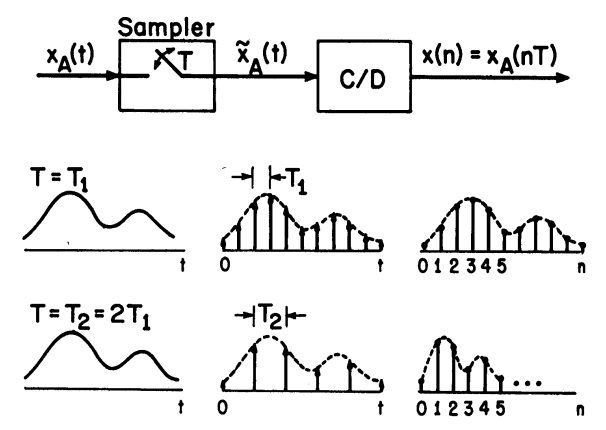
\includegraphics[width=0.7\linewidth]{img/img01}
	\end{center}
\end{frame}

\begin{frame}
	\begin{center}
		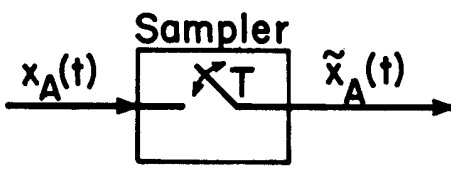
\includegraphics[width=0.3\linewidth]{img/img03}
	\end{center}
	\begin{itemize}
		\item The output of the sampler is the input to the sampler, multiplied by an impulse train:
		\[ \tilde{x}_A(t) = x_A(t)\sum_{- \infty}^{+\infty} u_o (t - nT) \]
		\item Or equivalently, an impulse train with the areas of the impulse given by the values of $ x_A(t) $ at the times that the impulses occur ($ nT $).
		\[ \tilde{x}_A(t) = \sum_{- \infty}^{+\infty} x_A(nT) u_o (t - nT) \]
	\end{itemize}
\end{frame}

\begin{frame}
	\begin{itemize}
		\item Then in the Fourier transformed domain, the continuous time Fourier transform, is the convolution of the continuous time Fourier transform of $ x_A(t) $, convolved with the Fourier transform of the impulse train, which is an impulse train in the frequency domain:
		\[ \tilde{X}_A(j\Omega) = X_A(j\Omega)*P(j\Omega) \]
		\item or equivalently:
		\[ \tilde{X}_A(j\Omega) = \frac{1}{T} \sum_{r = -\infty}^{+ \infty} X_A \left(j\Omega+j\frac{2 \pi r}{T}\right) \]
	\end{itemize}
\end{frame}

\begin{frame}
	\begin{itemize}
		\item So what that means is that the Fourier transform of continuous time signal, $ \tilde{x}_A(t) $, is equal to the Fourier transform of continuous time signal $ x_A(t) $, but repeated over and over again in frequency at intervals of $ \frac{2\pi}{T} $
	\end{itemize}
\end{frame}

\begin{frame}
	\begin{itemize}
		\item How about we look from a different point of view?
		\[ \tilde{X}_A(j\Omega) = \int\limits_{-\infty}^{+\infty} \tilde{X}_A(t) e^{-j \Omega t} dt \]
		\item Substitute in for $ \tilde{x}_A(t) $, the relationship in terms of an impulse train and interchange summation and integration
		\[ \tilde{X}_A(j\Omega) = \sum_{n = - \infty}^{+\infty} x_A(nT)  \int\limits_{-\infty}^{+\infty} e^{-j \Omega t} u_o (t - nT) dt \]
		\item then the Fourier transform at the output of the sampler as given by the sampling values times $ e^{-jn \Omega T} $.
		\[ \tilde{X}_A(j\Omega) = \sum_{n = - \infty}^{+\infty} x_A(nT)  e^{-jn\Omega T} \]
	\end{itemize}
\end{frame}

\begin{frame}
	\begin{center}
		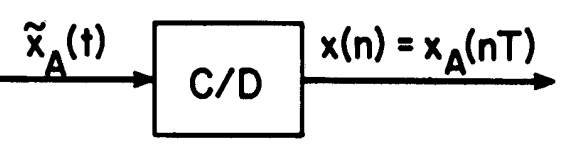
\includegraphics[width=0.4\linewidth]{img/img04}
	\end{center}
	\begin{itemize}
		\item We just developed two expression:
		\[ \tilde{X}_A(j\Omega) = \frac{1}{T} \sum_{r = -\infty}^{+ \infty} X_A \left(j\Omega+j\frac{2 \pi r}{T}\right) \] and 
		\[ \tilde{X}_A(j\Omega) = \sum_{n = - \infty}^{+\infty} x_A(nT)  e^{-jn\Omega T} \]
		\item What is the Fourier transform of the output of the continuous to discrete time converter?
		\[ X(e^{j\omega}) = \sum_n X_A(nT)e^{-j\omega n} \]
	\end{itemize}
\end{frame}

\begin{frame}
	\begin{itemize}
		\item Let's compare these two expressions:
		\[ \tilde{X}_A(j\Omega) = \sum_{n = - \infty}^{+\infty} x_A(nT)  e^{-jn\Omega T} \]
		\[ X(e^{j\omega}) = \sum_n X_A(nT)e^{-j\omega n} \]
		\item We see that they are exactly the same except that for $\omega$ and $\Omega T$
	\end{itemize}
\end{frame}

\begin{frame}
	\begin{itemize}
		\item Consequently, we can say that the discrete time Fourier transform is equal to the continuous time Fourier transform of the impulse train, with $ \Omega T $ equal to $\omega$
		\begin{align*}
			X(e^{j\omega}) &= \left.\tilde{X}_A(j\Omega)\right|_{\Omega T = \omega} \\
			&= \frac{1}{T} \sum_{r = -\infty}^{+ \infty} X_A \left(j\frac{\omega}{T}+j\frac{2 \pi r}{T}\right)
		\end{align*}
		\[  \]
	\end{itemize}
\end{frame}

\begin{frame}
	\begin{itemize}
		\item Relationship among the Fourier transforms of a continous-time signal, its samples, and the resulting sequence.
	\end{itemize}
	\begin{center}
		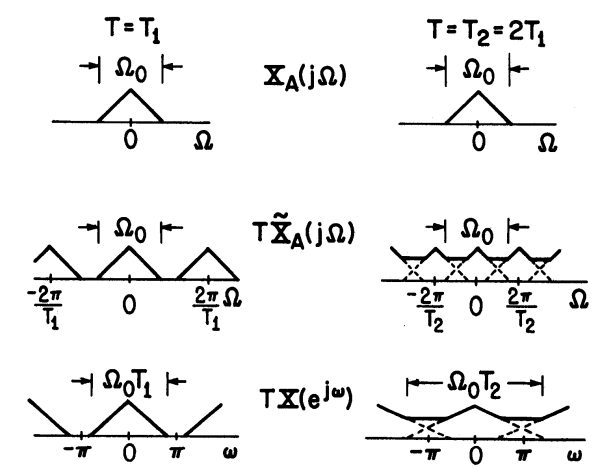
\includegraphics[width=0.6\linewidth]{img/img02}
	\end{center}
\end{frame}



\end{document}
